\section{Caracterización por respuesta al escalón (puntos extra)}
\label{sec:p7}
\enunciado{Caracterice el sistema mediante la respuesta al escalón (40\,\% extra). Adjunte un vídeo
de la respuesta al escalón (ejecutando la planta en físico con ustedes explicando y su
funcionamiento en computadora, debe ser un solo vídeo).}

\begin{center}
\textbf{Video del ensayo y su análisis en MATLAB:} \videoCaracterizacion
\end{center}

\subsection{Método}
Se usa un escalón del freno porque se puede aplicar de forma limpia y repetible; un impulso ideal
no es realizable, así que la respuesta al impulso se obtiene del modelo identificado (pregunta~1).
El motor acelera el disco, se corta, y tras un tramo de giro libre el servo pasa en una sola orden
de 120° a 180° y se mantiene. El ESP32 registra cada 20~ms el tiempo, el ángulo ordenado y la
velocidad en un archivo CSV.

El script \texttt{visualizar\_ensayo.m} ajusta una recta a la velocidad en los 300~ms anteriores y
posteriores al escalón. La pendiente previa $a_0$ es la caída libre por fricción. Suponiendo que el
freno añade una aceleración que crece como $K\Delta u\,(1-e^{-t/\tau})$, la velocidad predicha es
\[
  \widehat v(t)=v(0)+a_0t+K\Delta u\bigl[t-\tau(1-e^{-t/\tau})\bigr],\qquad t\geq 0,
\]
y $K$ y $\tau$ se ajustan por mínimos cuadrados hasta que el disco se detiene. El modelo
resultante, del ángulo del freno al cambio de velocidad respecto a la caída libre, es
\begin{equation}
  G(s)=\frac{K}{s(\tau s+1)},
  \label{eq:modelo_escalon}
\end{equation}
cuya respuesta al impulso se calcula con \texttt{tf} e \texttt{impulse} de MATLAB.

\subsection{Resultados}
El ensayo presentado (\texttt{escalon\_02}) tiene 500 muestras sin pérdidas. La
Fig.~\ref{fig:escalon02} muestra el escalón, la velocidad medida y el modelo ajustado, y la
Tabla~\ref{tab:caracterizacion} resume los resultados.

\begin{figure}[h]
\centering
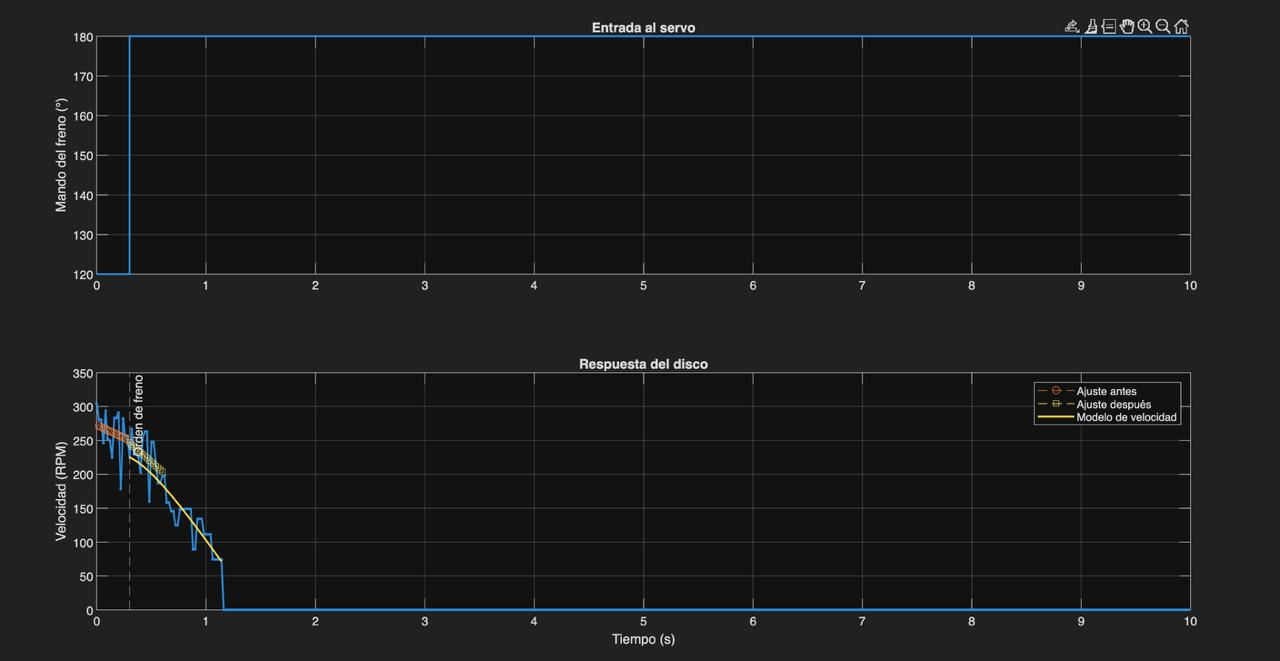
\includegraphics[width=\linewidth]{matlab_escalon_02.jpg}
\caption{Ensayo \texttt{escalon\_02}: orden al servo (arriba) y velocidad medida, rectas de
300~ms y modelo ajustado (abajo).}
\label{fig:escalon02}
\end{figure}

\begin{table}[h]
\centering\small
\caption{Resultados de la caracterización.}
\label{tab:caracterizacion}
\begin{tabular}{@{}lr@{}}
\toprule
Magnitud & Valor \\
\midrule
Velocidad al cortar el motor & $\approx 300$~RPM \\
Escalón $\Delta u$ & $120^\circ\to 180^\circ$ en $t=0{,}301$~s \\
Pendiente antes del freno & $-76{,}4$~RPM/s \\
Pendiente después del freno & $-142{,}9$~RPM/s \\
Ganancia $K$ & $-2{,}58$~(RPM/s)/grado \\
Constante de tiempo $\tau$ & $0{,}274$~s \\
RMSE del modelo & $25{,}0$~RPM \\
Detención del disco & $t\approx 1{,}14$~s \\
\bottomrule
\end{tabular}
\end{table}

Con estos valores,
\[
  G(s)=\frac{-2{,}58}{s\,(0{,}274\,s+1)}\ \frac{\text{RPM}}{\text{grado}},\qquad
  h(t)=-2{,}58\,\bigl(1-e^{-t/0{,}274}\bigr)\ \text{RPM},
\]
y la Fig.~\ref{fig:impulso02} muestra la respuesta al impulso obtenida con \texttt{impulse}.

\begin{figure}[h]
\centering
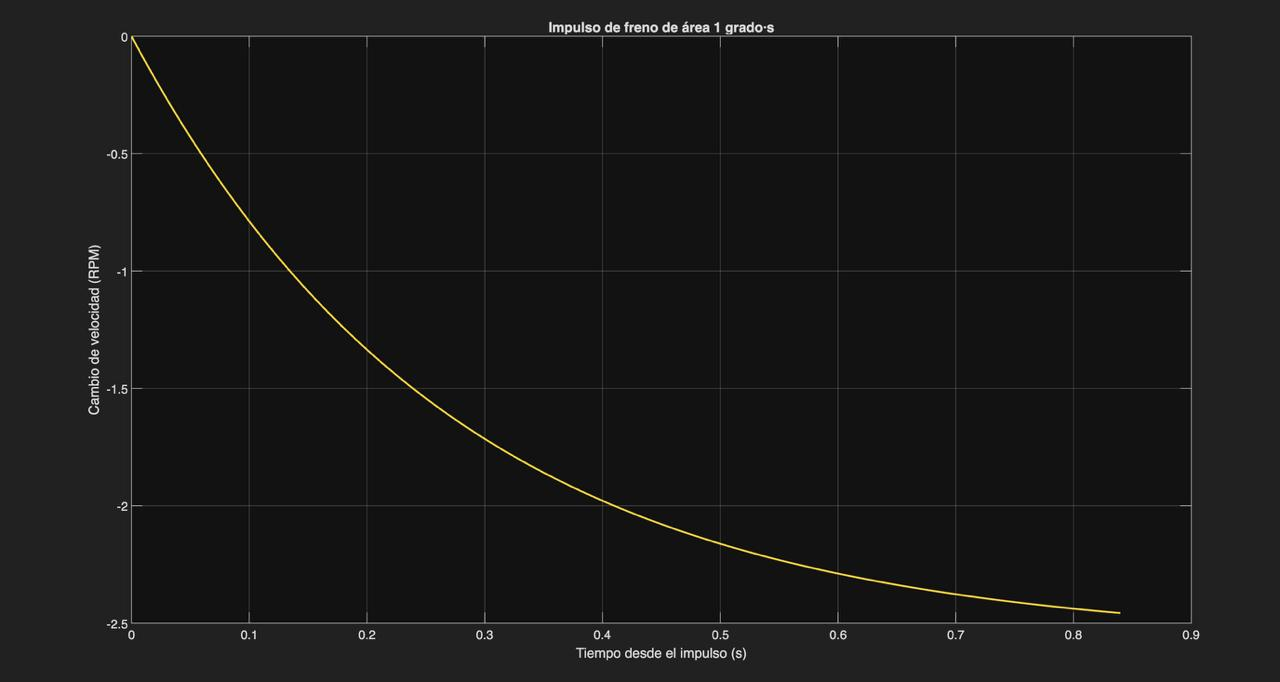
\includegraphics[width=0.8\linewidth]{matlab_impulso_02.jpg}
\caption{Respuesta al impulso del modelo identificado (impulso de 1 grado$\cdot$s).}
\label{fig:impulso02}
\end{figure}

\subsection{Análisis}
El freno casi duplica la desaceleración, de $-76$ a $-143$~RPM/s, y $K<0$ confirma que más ángulo
de freno quita velocidad. El resultado es coherente con el modelo de la pregunta~5: la caída libre
corresponde a los términos de fricción, que el método resta, y el efecto del freno no es
instantáneo sino que crece con $\tau=0{,}27$~s, que incluye el recorrido del servo y el tiempo de
contacto de la goma. Si $\tau\to 0$, la ec.~\eqref{eq:modelo_escalon} se reduce a la forma de la
pregunta~5 con $K=-K_f/J_\text{eq}$. El RMSE de 25~RPM proviene principalmente del ruido del
sensor, que produce saltos entre muestras. El modelo es local: es válido cerca de 300~RPM y para
este escalón, y debe validarse con otros ensayos antes de diseñar el PID.
